\documentclass[../piano-di-qualifica.tex]{subfiles}

\begin{document}

\subsection{Test di accettazione}
\label{sub:test_di_accettazione}
Dimostrano che il prodotto è in grado di soddisfare i requisiti minimi concordati con il proponente.
I test di accettazione si relazionano con i test di sistema e vengono eseguiti durante il collaudo finale del prodotto, sia dai membri del team che dal proponente sotto la supervisione del team.



%inizio tabella test di accettazione
\rowcolors{2}{white!80!lightgray!90}{white}
\renewcommand{\arraystretch}{2} % 
\begin{longtable}[H]{>{\centering\bfseries}m{2.5cm} >{\centering}m{7.5cm} >{\centering}m{2.5cm} >{\centering\arraybackslash}m{3.5cm}}
  \caption{Tabella test di accettazione}%
  \label{tab:tabella_test_di_accettazione}                                                    \\
  \rowcolor{lightgray}
  {\textbf{Requisito}} & {\textbf{Descrizione}} & {\textbf{Priorità}} & {\textbf{Implementazione}}  \\
  \endfirsthead%
  \rowcolor{lightgray}
  {\textbf{Requisito}} & {\textbf{Descrizione}} & {\textbf{Priorità}} & {\textbf{Implementazione}}  \\
  \endhead%
  \rowcolor{white}
  \multicolumn{4}{c}{\textit{Continua alla pagina successiva}}
  \endfoot%
  \endlastfoot%
  \textbf{TARFO1} & Si verifica che l'utente possa addestrare il sistema inserendo i dati tramite degli appositi pulsanti. & Obbligatorio & Non Implementato \\

  \textbf{TARFD1.1.1} & Si verifica che si venga notificati con un messaggio d’errore nel caso si carichino i dati di addestramento in un formato non valido. & Desiderabile & Non Implementato \\
  
  \textbf{TARFD1.2.1} & Si verifica che l’utente venga notificato con un messaggio d’errore nel caso si carichi un predittore in un formato non valido. & Desiderabile & Non Implementato \\
  
  \textbf{TARFO1.3} & Si verifica che l'utente possa scegliere il modello di machine learning per l'addestramento. & Obbligatorio & Non Implementato \\
  
  \textbf{TARFO1.4} & Si che verifica che l'utente possa avviare l'addestramento & Obbligatorio & Non Implementato \\
  \textbf{TARFO1.5} & Si verifica che l'utente abbia a disposizione un pulsante per il caricamento di un file \glossario{JSON} contenente il \glossario{predittore} allenato in precedenza. & Obbligatorio & Non Implementato \\
  
  \textbf{TARFF2} & Si verifica che l'utente possa addestrare il sistema direttamente da Grafana & Facoltativo & Non Implementato \\
  
  \textbf{TARFF3} & Si verifica che l'utente possa avviare l'apprendimento del flusso di dati costante per mezzo di un pannello. & Facoltativo & Non Implementato \\
  \textbf{TARFF4} & Si verifica che l'utente possa disattivare l'apprendimento del flusso di dati costante per mezzo di un pannello. & Facoltativo & Non Implementato \\
  \textbf{TARFO5} & Si verifica che l'utente possa configurare il plug-in. & Obbligatorio & Non Implementato \\
  \textbf{TARFO5.1} & Si verifica che l'utente abbia a disposizione un metodo per caricare il modello addestrato. & Obbligatorio & Non Implementato \\
  \textbf{TARFD5.1.1} & Si verifica che l'utente venga notificato con un messaggio d'errore nel caso in cui venga caricato un file contenente il modello addestrato non valido. & Desiderabile & Non Implementato \\
  \textbf{TARFD5.1.2} & Si verifica che l'utente venga notificato con un messaggio d'errore nel caso in cui non venga caricato nessun file. & Desiderabile & Non Implementato \\
  \textbf{TARFO5.2} & Si verifica che l'utente possa selezionare i nodi su cui desidera effettuare la predizione. & Obbligatorio & Non Implementato \\
  \textbf{TARFD5.2.1} & Si verifica che l'utente venga notificato con un messaggio d'errore nel caso in cui venga selezionato un nodo non valido. & Desiderabile & Non Implementato \\
  \textbf{TARFD5.2.2} & Si verifica che l'utente venga notificato con un messaggio d'errore nel caso in cui non venga selezionato alcun nodo. & Desiderabile & Non Implementato \\
  \textbf{TARFO5.3} & Si verifica che l'utente possa selezionare il tipo di visualizzazione della predizione. & Obbligatorio & Non Implementato \\
  \textbf{TARFD5.3.1} & Si verifica che l'utente venga notificato con un messaggio d'errore nel caso in cui non venga selezionato alcun tipo di visualizzazione. & Desiderabile & Non Implementato \\
  \textbf{TARFO6} & Si verifica che l'utente abbia a disposizione la possibilità di visualizzare la previsione utilizzando un grafico. & Obbligatorio & Non Implementato \\
  \textbf{TARFO7} & Si verifica che l'utente abbia a disposizione la possibilità di visualizzare la previsione utilizzando un indicatore. & Obbligatorio & Non Implementato \\
  \textbf{TARFO8} & Si verifica che l'utente possa selezionare il modello SVM per l'allenamento. & Obbligatorio & Non Implementato \\
  \textbf{TARFO9} & Si verifica che l'utente possa selezionare il modello RL per l'allenamento. & Obbligatorio & Non Implementato \\
  \textbf{TARFF10} & Si verifica che l'utente possa selezionare la regressione esponenziale per l'allenamento. & Facoltativo & Non Implementato \\
  \textbf{TARFF11} & Si verifica che l'utente possa selezionare la regressione logaritmica per l'allenamento. & Facoltativo & Non Implementato \\
  \textbf{TARFF12} & Si verifica che l'utente possa selezionare il modello rete neurale per l'allenamento. & Facoltativo & Non Implementato \\
  \textbf{TARFF13} & Si verifica che l'utente possa selezionare il modello SVM adattata alla regressione per l'allenamento. & Facoltativo & Non Implementato \\
  \textbf{TARFO14} & Si verifica che l'utente abbia a disposizione un pulsante per l’avvio della predizione. & Obbligatorio & Non Implementato \\
  \textbf{TARFO15} & Si verifica che l'utente abbia a disposizione un pulsante per interrompere la predizione. & Obbligatorio & Non Implementato \\
  \textbf{TARFF16} & Si verifica che all'utente venga mostrato il pannello contenente le informazioni riguardanti la bontà della previsione. & Facoltativo & Non Implementato \\
  \textbf{TARFF17} & Si verifica che all'utente venga mostrato il pannello contenente la bontà di previsione dell'algoritmo SVM descritta dal parametro F-Measure. & Facoltativo & Non Implementato \\
  \textbf{TARFF18} & Si verifica che all'utente venga mostrato il pannello contenente la bontà di previsione dell'algoritmo RL descritta dal parametro R\textsuperscript{2}. & Facoltativo & Non Implementato \\
  \textbf{TARFF19} & Si verifica che l'utente abbia a disposizione un metodo per l’impostazione degli alert. & Facoltativo & Non Implementato \\
  \textbf{TARFF19.1} & Si verifica che all'utente venga mostrato un pulsante che permetta all'utente di creare un alert. & Facoltativo & Non Implementato \\
  \textbf{TARFF19.2} & Si verifica che l'utente abbia a disposizione un sistema per inserire una soglia di alert. & Facoltativo & Non Implementato \\
  \textbf{TARFD19.2.1} & Si verifica che l'utente venga notificato un messaggio di errore nel caso in cui venga superata la soglia impostata utilizzando un allert. & Desiderabile & Non Implementato \\
  \textbf{TARFD20} & Si verifica che l'utente possa eliminare il pannello di monitoraggio. & Desiderabile & Non Implementato \\
  \textbf{TARFD20.1} & Si verifica che l'utente visualizzi un messaggio di errore nel caso in cui si cerchi di eliminare il pannello senza interrompere la previsione. & Desiderabile & Non Implementato \\
  \textbf{TARFO21} & Si verifica che l'utente abbia a disposizione un metodo per la visualizzazione delle previsioni. & Obbligatorio & Non Implementato \\
\end{longtable}




\subsection{Test di sistema}
\label{sub:test_di_sistema}
Garantiscono che i requisiti richiesti identificati nel documento \textsc{Analisi dei Requisiti v1.9-1.3.0} vengano soddisfatti.

%inizio tabella test di sistema
\rowcolors{2}{white!80!lightgray!90}{white}
\renewcommand{\arraystretch}{2} % 
\begin{longtable}[H]{>{\centering\bfseries}m{2.5cm} >{\centering}m{7.5cm} >{\centering}m{2.5cm} >{\centering\arraybackslash}m{3.5cm}}
  \caption{Tabella test di sistema}%
  \label{tab:tabella_test_di_sistema}                                                    \\
  \rowcolor{lightgray}
  {\textbf{Requisito}} & {\textbf{Descrizione}} & {\textbf{Priorità}} & {\textbf{Implementazione}}  \\
  \endfirsthead%
  \rowcolor{lightgray}
  {\textbf{Requisito}} & {\textbf{Descrizione}} & {\textbf{Priorità}} & {\textbf{Implementazione}}  \\
  \endhead%
  \rowcolor{white}
  \multicolumn{4}{c}{\textit{Continua alla pagina successiva}}
  \endfoot%
  \endlastfoot%
  \textbf{TSRFO1} & Si verifica che l'utente possa addestrare il sistema inserendo i dati tramite degli appositi pulsanti. & Obbligatorio & Implementato \\

  \textbf{TSRFD1.1.1} & Si verifica che si venga notificati con un messaggio d’errore nel caso si carichino i dati di addestramento in un formato non valido. & Desiderabile & Implementato \\

  \textbf{TSRFD1.2.1} & Si verifica che l’utente venga notificato con un messaggio d’errore nel caso si carichi un predittore in un formato non valido. & Desiderabile & Implementato \\
  
  \textbf{TSRFO1.3} & Si verifica che l'utente possa scegliere il modello di machine learning per l'addestramento. & Obbligatorio & Implementato \\

  \textbf{TSRFO1.4} & Si che verifica che l'utente possa avviare l'addestramento & Obbligatorio & Implementato \\
  \textbf{TSRFO1.5} & Si verifica che l'utente abbia a disposizione un pulsante per il caricamento di un file \glossario{JSON} contenente il \glossario{predittore} allenato in precedenza. & Obbligatorio & Implementato \\
  
  \textbf{TSRFF2} & Si verifica che l'utente possa addestrare il sistema direttamente da Grafana & Facoltativo & Non Implementato \\
  
  \textbf{TSRFF3} & Si verifica che l'utente possa avviare l'apprendimento del flusso di dati costante per mezzo di un pannello. & Facoltativo & Non Implementato \\
  \textbf{TSRFF4} & Si verifica che l'utente possa disattivare l'apprendimento del flusso di dati costante per mezzo di un pannello. & Facoltativo & Non Implementato \\
  \textbf{TSRFO5} & Si verifica che l'utente possa configurare il plug-in. & Obbligatorio & Implementato \\
  \textbf{TSRFO5.1} & Si verifica che l'utente abbia a disposizione un metodo per caricare il modello addestrato. & Obbligatorio & Implementato \\
  \textbf{TSRFD5.1.1} & Si verifica che l'utente venga notificato con un messaggio d'errore nel caso in cui venga caricato un file contenente il modello addestrato non valido. & Desiderabile & Non Implementato \\
  \textbf{TSRFD5.1.2} & Si verifica che l'utente venga notificato con un messaggio d'errore nel caso in cui non venga caricato nessun file. & Desiderabile & Implementato \\
  \textbf{TSRFO5.2} & Si verifica che l'utente possa selezionare i nodi su cui desidera effettuare la predizione. & Obbligatorio & Implementato \\
  \textbf{TSRFD5.2.1} & Si verifica che l'utente venga notificato con un messaggio d'errore nel caso in cui venga selezionato un nodo non valido. & Desiderabile & Implementato \\
  \textbf{TSRFD5.2.2} & Si verifica che l'utente venga notificato con un messaggio d'errore nel caso in cui non venga selezionato alcun nodo. & Desiderabile & Implementato \\
  \textbf{TSRFO5.3} & Si verifica che l'utente possa selezionare il tipo di visualizzazione della predizione. & Obbligatorio & Implementato \\
  \textbf{TSRFD5.3.1} & Si verifica che l'utente venga notificato con un messaggio d'errore nel caso in cui non venga selezionato alcun tipo di visualizzazione. & Desiderabile & Non Implementato \\
  \textbf{TSRFO6} & Si verifica che l'utente abbia a disposizione la possibilità di visualizzare la previsione utilizzando un grafico. & Obbligatorio & Implementato \\
  \textbf{TSRFO7} & Si verifica che l'utente abbia a disposizione la possibilità di visualizzare la previsione utilizzando un indicatore. & Obbligatorio & Implementato \\
  \textbf{TSRFO8} & Si verifica che l'utente possa selezionare il modello SVM per l'allenamento. & Obbligatorio & Implementato \\
  \textbf{TSRFO9} & Si verifica che l'utente possa selezionare il modello RL per l'allenamento. & Obbligatorio & Implementato \\
  \textbf{TSRFF10} & Si verifica che l'utente possa selezionare la regressione esponenziale per l'allenamento. & Facoltativo & Non Implementato \\
  \textbf{TSRFF11} & Si verifica che l'utente possa selezionare la regressione logaritmica per l'allenamento. & Facoltativo & Non Implementato \\
  \textbf{TSRFF12} & Si verifica che l'utente possa selezionare il modello rete neurale per l'allenamento. & Facoltativo & Non Implementato \\
  \textbf{TSRFF13} & Si verifica che l'utente possa selezionare il modello SVM adattata alla regressione per l'allenamento. & Facoltativo & Non Implementato \\
  \textbf{TSRFO14} & Si verifica che l'utente abbia a disposizione un pulsante per l’avvio della predizione. & Obbligatorio & Implementato \\
  \textbf{TSRFO15} & Si verifica che l'utente abbia a disposizione un pulsante per interrompere la predizione. & Obbligatorio & Implementato \\
  \textbf{TSRFF16} & Si verifica che all'utente venga mostrato il pannello contenente le informazioni riguardanti la bontà della previsione. & Facoltativo & Non Implementato \\
  \textbf{TSRFF17} & Si verifica che all'utente venga mostrato il pannello contenente la bontà di previsione dell'algoritmo SVM descritta dal parametro F-Measure. & Facoltativo & Non Implementato \\
  \textbf{TSRFF18} & Si verifica che all'utente venga mostrato il pannello contenente la bontà di previsione dell'algoritmo RL descritta dal parametro R\textsuperscript{2}. & Facoltativo & Non Implementato \\
  \textbf{TSRFF19} & Si verifica che l'utente abbia a disposizione un metodo per l’impostazione degli alert. & Facoltativo & Non Implementato \\
  \textbf{TSRFF19.1} & Si verifica che all'utente venga mostrato un pulsante che permetta all'utente di creare un alert. & Facoltativo & Non Implementato \\
  \textbf{TSRFF19.2} & Si verifica che l'utente abbia a disposizione un sistema per inserire una soglia di alert. & Facoltativo & Non Implementato \\
  \textbf{TSRFD19.2.1} & Si verifica che l'utente venga notificato un messaggio di errore nel caso in cui venga superata la soglia impostata utilizzando un alert. & Desiderabile & Non Implementato \\
  \textbf{TSRFD20} & Si verifica che l'utente possa eliminare il pannello di monitoraggio. & Desiderabile & Implementato \\
  \textbf{TSRFD20.1} & Si verifica che l'utente visualizzi un messaggio di errore nel caso in cui si cerchi di eliminare il pannello senza interrompere la previsione. & Desiderabile & Non Implementato \\
  \textbf{TSRFO21} & Si verifica che l'utente abbia a disposizione un metodo per la visualizzazione delle previsioni. & Obbligatorio & Implementato \\

\end{longtable}

\subsection{Test di integrazione}
\label{sub:test_di_integrazione}
Garantiscono il corretto funzionamento di ogni componente del sistema quando viene integrata con le altre.

%inizio tabella test di integrazione
\rowcolors{2}{white!80!lightgray!90}{white}
\renewcommand{\arraystretch}{2} % 
\begin{longtable}[H]{>{\centering\bfseries}m{2.5cm} >{\centering}m{7.5cm} >{\centering\arraybackslash}m{3.5cm}}
  \caption{Tabella test di integrazione}%
  \label{tab:tabella_test_di_integrazione}                                                    \\
  \rowcolor{lightgray}
  {\textbf{Test}} & {\textbf{Descrizione}} & {\textbf{Implementazione}}  \\
  \endfirsthead%
  \rowcolor{lightgray}
  {\textbf{Test}} & {\textbf{Descrizione}} & {\textbf{Implementazione}}  \\
  \endhead%
  \rowcolor{white}
  \multicolumn{3}{c}{\textit{Continua alla pagina successiva}}
  \endfoot%
  \endlastfoot%
  \textbf{TI1} & Si verifica il corretto caricamento del file CSV nel programma. & Implementato \\
  \textbf{TI2} & Si verifica la correttezza del grafico che viene visualizzato una volta caricato i dati. & Implementato \\
  \textbf{TI3} & Si verifica la correttezza dei coefficenti calcolati. & Implementato \\
  \textbf{TI4} & Si verifica la correttezza della struttura del file JSON una volta salvato. & Implementato \\
  \textbf{TI5} & Si verifica che il plug-in di Grafana carichi correttamente i dati. & Implementato \\

\end{longtable}

\subsection{Test di unità}
\label{sub:test_di_unita}
Garantiscono il corretto funzionamento di ogni minimo componente autonomo del sistema.

%inizio tabella test di integrazione
\rowcolors{2}{white!80!lightgray!90}{white}
\renewcommand{\arraystretch}{2} % 
\begin{longtable}[H]{>{\centering\bfseries}m{2.5cm} >{\centering}m{7.5cm} >{\centering\arraybackslash}m{3.5cm}}
  \caption{Tabella test di unità}%
  \label{tab:tabella_test_di_unita}                                                    \\
  \rowcolor{lightgray}
  {\textbf{Test}} & {\textbf{Descrizione}} & {\textbf{Implementazione}}  \\
  \endfirsthead%
  \rowcolor{lightgray}
  {\textbf{Test}} & {\textbf{Descrizione}} & {\textbf{Implementazione}}  \\
  \endhead%
  \rowcolor{white}
  \multicolumn{3}{c}{\textit{Continua alla pagina successiva}}
  \endfoot%
  \endlastfoot%
  \textbf{TU1} & Viene verificato il corretto avviamento dell'applicazione & Implementato \\
  \textbf{TU2} & Viene verificata la corretta lettura dei dati del file CVS inserito dall'utente & Implementato \\
  \textbf{TU3} & Viene verificata la corretta lettura dei dati del file predittore inserito dall'utente & Implementato \\
  \textbf{TU4} & Viene verificato che il costruttore dalla View costruisca la View come definito & Implementato \\
  \textbf{TU5} & Viene verificato che la funzione bindFileChange(handler) della View venga eseguita correttamente quando viene aggiunto un nuovo file CVS & Implementato \\
  \textbf{TU6} & Viene verificato che la funzione bindLoadPredictor(handler) della View venga eseguita correttamente quando viene aggiunto un nuovo file predittore & Implementato \\
  \textbf{TU7} & Viene verificato che la funzione bindFormSubmit(handler) della View venga eseguita correttamente quando viene cliccato il pulsante "Salva" & Implementato \\
  \textbf{TU8} & Viene verificato che la funzione addRlLine(coeff, min, max) della View venga eseguita correttamente per creare la retta della regressione lineare & Non Implementato \\
  \textbf{TU9} & Viene verificato che la funzione buildPage(json) della View venga eseguita correttamente per ricaricare la pagina in caso di modifiche alle opzioni di selezione da parte dell'utente & Non Implementato \\
  \textbf{TU10} & Viene verificato che la funzione showContent() della View cambi correttamente lo stato di visibilità di un elemento della form & Implementato \\
  \textbf{TU11} & Viene verificato che la funzione showChart() della View cambi correttamente lo stato di visibilità del grafico generato & Implementato \\
  \textbf{TU12} & Viene verificato che la funzione hideContent() della View cambi correttamente lo stato di visibilità di un elemento della form & Implementato \\
  \textbf{TU13} & Viene verificato che la funzione hideChart() della View cambi correttamente lo stato di visibilità del grafico generato & Implementato \\
  \textbf{TU14} & Viene verificato che la funzione initSelectTarget(json) della View inserisca correttamente la variabile target & Implementato \\
  \textbf{TU15} & Viene verificato che la funzione initVars(json) della View inserisca correttamente la variabili contenute nel file CVS & Non Implementato \\
  \textbf{TU16} & Viene verificato che la funzione addVar(key) della View inserisca correttamente le label delle variabili all'interno dell'interfaccia grafica & Implementato \\
  \textbf{TU17} & Viene verificato che la funzione addTarget(key) della View specifichi correttamente quale variabile è stata selezionata come target & Implementato \\
  \textbf{TU18} & Viene verificato che la funzione getTarget() della View ritorni correttamente quale variabile è stata selezionata come target & Implementato \\
  \textbf{TU19} & Viene verificato che la funzione getVars() della View ritorni correttamente quali variabili sono state selezionate dall'utente & Implementato \\
  \textbf{TU20} & Viene verificato che la funzione setNotes(notes) della View inserisca correttamente le note inserite dall'utente & Implementato \\
  \textbf{TU21} & Viene verificato che la funzione showError(message) della View mostri il messaggio di errore corretto per un qualsiasi caso & Implementato \\
  \textbf{TU22} & Viene verificato che la funzione reset() della View resetti la form dell'interfaccia grafica & Non Implementato \\
  \textbf{TU23} & Viene verificato che la funzione getNotes() della View ritorni le note inserite dall'utente & Implementato \\
  \textbf{TU24} & Viene verificato che la funzione updateChart() della View aggiorni correttamente il grafico & Non Implementato \\
  \textbf{TU25} & Viene verificato che la funzione getChartX() della View ritorni i dati dell'asse X & Implementato \\
  \textbf{TU26} & Viene verificato che la funzione getChartY() della View ritorni i dati dell'asse Y & Implementato \\
  \textbf{TU27} & Viene verificato che la funzione getChartTargetArray() della View ritorni i dati della variabile target presi dal grafico & Implementato \\
  \textbf{TU28} & Viene verificato che la funzione setChartData(x, y, target, xLabel, yLabel, model) della View inserisca correttamente i nuovi dati nel grafico & Implementato \\
  \textbf{TU29} & Viene verificato che il costruttore dal Controller definisca correttamente i bind con la View & Implementato \\
  \textbf{TU30} & Viene verificato che la funzione handleFileChanged(path) del Controller venga attivata dopo l'esecuzione della funzione bindFileChange(handler) della View & Non Implementato \\
  \textbf{TU31} & Viene verificato che la funzione handleFormSubmit(keys, meta) del Controller venga attivata dopo l'esecuzione della funzione bindFormSubmit(handler) della View & Non Implementato \\
  \textbf{TU32} & Viene verificato che la funzione handleLoadPredictor(path) del Controller venga attivata dopo l'esecuzione della funzione bindLoadPredictor(handler) della View & Non Implementato \\
  \textbf{TU33} & Viene verificato che la funzione readFromCVS(path) del Model legga correttamente i dati dal file CVS instanziando un oggetto CVSFile & Implementato \\
  \textbf{TU34} & Viene verificato che la funzione convertCVStoJSON() del Model converta un oggetto CVSFile in un oggetto JSONFile & Non Implementato \\
  \textbf{TU35} & Viene verificato che la funzione getDataByFilter(param) del Model ritorni i dati filtrati per certi parametri & Non Implementato \\
  \textbf{TU36} & Viene verificato che la funzione loadPredictor(path) del Model carichi i dati di un predittore in un oggetto JSONFile & Non Implementato \\
  \textbf{TU37} & Viene verificato che la funzione get notes() del Model ritorni le note contenuto nel modello dei dati & Implementato \\
  \textbf{TU38} & Viene verificato che la funzione get json() del Model ritorni il file JSON salvato & Implementato \\
  \textbf{TU39} & Viene verificato che la funzione calculatePredictor(data, meta) del Model ritorni correttamente le informazioni con i dati allenati & Implementato \\
  \textbf{TU40} & Viene verificato che la funzione savePredictor(pred) del Model salvi correttamente il file predittore sul computer dell'utente & Non Implementato \\
  \textbf{TU41} & Viene verificato che quando viene estesa l'interfaccia modelTrain, venga restituito un errore nel caso non sia stato implementato il metodo executeTraining(data) & Non Implementato \\
  \textbf{TU42} & Viene verificato che il costruttore di RLadapter instanzi correttamente l'oggetto di tipo regressione & Implementato \\
  \textbf{TU43} & Viene verificato che la funzione calculateMatrixDimensions(data) di RLadapter ritorni la corretta dimensione della matrice dei dati & Implementato \\
  \textbf{TU44} & Viene verificato che la funzione libAdaptation(data, matrix, reg) di RLadapter inserisca correttamente i dati di predizione all'interno dell'oggetto di regressione lineare & Implementato \\
  \textbf{TU45} & Viene verificato che la funzione generateRLOutput(data, coefficients) di RLadapter ritorni correttamente i dati allenati e conformi per l'inserimento nel predittore & Implementato \\
  \textbf{TU46} & Viene verificato che la funzione executeTraining(data) di RLadapter ritorni correttamente i dati allenati & Implementato \\
  \textbf{TU47} & Viene verificato che il costruttore di SVMadapter instanzi correttamente l'oggetto di tipo svm & Implementato \\
  \textbf{TU48} & Viene verificato che la funzione calculateMatrixDimensions(data) di SVMadapter ritorni la corretta dimensione della matrice dei dati & Implementato \\
  \textbf{TU49} & Viene verificato che la funzione splitData(data,matrix) di SVMadapter dividi correttamente i dati tra variabili e labels & Implementato \\
  \textbf{TU50} & Viene verificato che la funzione executeTraining(data) di SVMadapter ritorni correttamente i dati allenati & Implementato \\
  \textbf{TU51} & Viene verificato che la funzione bindFormSubmit(handler) della View esponga il messaggio di errore 'Target cannot be in variables list' nel caso la variabile selezionata non possa essere target  & Implementato \\
  \textbf{TU52} & Viene verificato che la funzione bindFormSubmit(handler) della View esponga il messaggio di errore 'Select at least one valid variable' nel caso si fosse selezionato varie variabili ma non quella target  & Implementato \\
  \textbf{TU53} & Viene verificato che la funzione bindFormSubmit(handler) della View esponga il messaggio di errore 'Select a target' nel caso non si selezioni una variabile target & Implementato \\
  \textbf{TU54} & Viene verificato che si visualizzi un messaggio di errore nel caso in cui il caricamento del file JSON nel plug-in non vada a buon fine & Implementato \\
  \textbf{TU55} & Viene verificato che si visualizzi un messaggio di errore nel caso in cui nel plug-in non venga selezionato alcun file JSON & Implementato \\
  \textbf{TU56} & Viene verificato che si visualizzi un messaggio quando il caricamento del file JSON nel plug-in è andato a buon fine & Implementato \\
  \textbf{TU57} & Viene verificato che il file JSON venga letto correttamente nel caso si selezioni la RL nel plug-in & Implementato \\
  \textbf{TU58} & Viene verificato che il file JSON venga letto correttamente nel caso si selezioni la SVM nel plug-in & Implementato \\
  \textbf{TU59} & Viene verificato che il metodo del plug-in predict di PredictionRL ritorni i valori corretti & Implementato \\
  \textbf{TU60} & Viene verificato che il metodo del plug-in predict di PredictionSVM ritorni i valori corretti & Implementato \\
\end{longtable}

\begin{figure}[H]
  \centering
  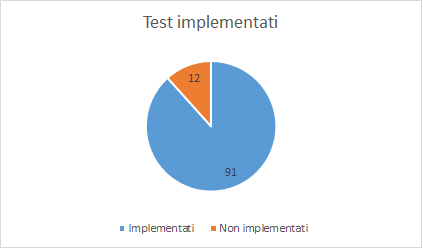
\includegraphics[width=10cm]{img/testImplementati.png}
  \label{fig:test_implementati}
  \caption{Grafico con i test implementati}
\end{figure}

\end{document}